\appendix 

\chapter{Przykładowe aplikacje}

Zapraszam do przeglądu interesujących przykładowych programów, które z różnych względów nie znalazły się
wśród programów przedstawianych wcześniej. Każdy z tych programów demostruje różne przydatne techniki
bądź programistyczne związane z platformą .NET. Programy pozostawię bez komentarza, aby
czytelnik mógł przeanalizować je samodzielnie.

\section{Animowany fraktalny zbiór Julii}

\begin{figure}
\begin{center}
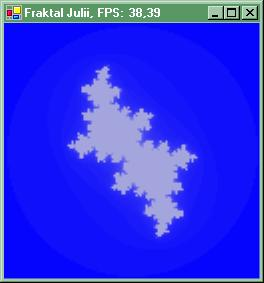
\includegraphics[width=0.50\textwidth]{./pic/app01}
\caption{Animowany fraktalny zbiór Julii}
\end{center}
\end{figure}

\begin{scriptsize}
\begin{verbatim}
using System;
using System.Drawing;
using System.Drawing.Imaging;
using System.Windows.Forms;
using System.Runtime.InteropServices; 

namespace vicMazeGen
{
  public class CFrmJulia : System.Windows.Forms.Form
  {
    private const int PSiz = 128;
    
    private double angle = 0.0, angle2 = 0.0;
    private int    cx, cy;

    private Bitmap picFracSource;
    private System.Windows.Forms.PictureBox picFrac;

    public CFrmJulia()
    {
      this.SetStyle(ControlStyles.DoubleBuffer, true);
      this.SetStyle(ControlStyles.AllPaintingInWmPaint, true);

      picFracSource = new Bitmap( PSiz, PSiz, PixelFormat.Format24bppRgb );

      this.picFrac = new System.Windows.Forms.PictureBox();
      this.picFrac.Dock = DockStyle.Fill;
      this.picFrac.SizeMode = System.Windows.Forms.PictureBoxSizeMode.StretchImage;

      this.ClientSize = new System.Drawing.Size(256, 256);
      this.StartPosition = System.Windows.Forms.FormStartPosition.CenterScreen;

      this.Controls.Add( this.picFrac );
    }

    void JuliaPaint()
    {
      angle += 0.023; angle2+= 0.027;
      cx = (int)( 800.0 * Math.Sin( angle+1.0 ) ); 
      cy = (int)( 800.0 * Math.Cos( angle2 ) );

      Rectangle bounds = 
        new Rectangle( new Point(0, 0), 
        new Size( picFracSource.Width, picFracSource.Height ) ); 
      BitmapData bData = 
        picFracSource.LockBits( bounds, ImageLockMode.ReadWrite, 
                                PixelFormat.Format24bppRgb );

      byte[] picData = new byte[PSiz * PSiz * 3];
      int iDex = 0;

      int iterNo, i, j;
      int x, y, xn, yn, x2, y2;
      for (i=0; i<PSiz; i++ )
        for (j=0; j<PSiz; j++ )
        {
          iterNo = 0;
          
          x  = (i<<5)-2048; 
          y  = (j<<5)-2048;
          x2 = x*x;  
          y2 = y*y;
          while ( 
                  ( iterNo++ < 32 ) && 
                  ( Math.Abs(x2+y2) < 4000000 ) 
                )
          {
            x2 = x*x; y2 = y*y;
            xn = ((x2-y2)>>10) + cx;
            yn = ((x*y)>>9)    + cy;
            x  = xn; y  = yn;
          }

          picData[iDex++] = Convert.ToByte(255-iterNo);
          picData[iDex++] = Convert.ToByte(5*iterNo);
          picData[iDex++] = Convert.ToByte(5*iterNo);
        }

      Marshal.Copy ( picData, 0, bData.Scan0, PSiz * PSiz * 3 ); 
      picFracSource.UnlockBits( bData );

      this.picFrac.Image = picFracSource; 
      this.picFrac.Invalidate();
    }

    public static void Main()
    {
      CFrmJulia frm = new CFrmJulia(); 
      frm.Show();
  
      DateTime start = DateTime.Now;
      int      frame = 0;
      while ( frm.Created )
      {
        frm.JuliaPaint();
        Application.DoEvents();

        frm.Text = String.Format( "Fraktal Julii, FPS: {0:N}", 
                   frame/((TimeSpan)(DateTime.Now-start)).TotalSeconds );      
        frame++;
      } 
    }
  }
}
\end{verbatim}
\end{scriptsize}

\section{Bezpośredni dostęp do nośnika danych w Windows NT}

\begin{scriptsize}
\begin{verbatim}
#include <windows.h>
#include <stdio.h>

void ShowErrorMessage()
{
  char* lpMsgBuf;
  FormatMessage( 
    FORMAT_MESSAGE_ALLOCATE_BUFFER | FORMAT_MESSAGE_FROM_SYSTEM,
    NULL,
    GetLastError(),
    MAKELANGID(LANG_NEUTRAL, SUBLANG_DEFAULT), 
    (LPTSTR) &lpMsgBuf,
    0,
    NULL 
    );

  // Pokaż komunikat
  MessageBox( NULL, lpMsgBuf, "GetLastError", MB_OK|MB_ICONINFORMATION );

  // Zwolnij pamięć
  LocalFree( lpMsgBuf );

  exit( 1 );
}

int main( int argc, char **argv )
{
  BOOL bResult;

  const int nBytesToRead = 512;
  unsigned long nBytesRead;
  unsigned long nBytesWrote;
  char  inBuffer[nBytesToRead];

  HANDLE hFloppy = CreateFile( "\\\\.\\a:", 
      GENERIC_WRITE | GENERIC_READ, 
      FILE_SHARE_READ | FILE_SHARE_WRITE,
      NULL, OPEN_EXISTING, 0, NULL );
  if ( hFloppy == INVALID_HANDLE_VALUE ) ShowErrorMessage();

  HANDLE hData = CreateFile( "read.bin", 
       GENERIC_READ | GENERIC_WRITE, 
       FILE_SHARE_READ | FILE_SHARE_WRITE,
       NULL, CREATE_ALWAYS, 0, NULL );  
  if ( hData == INVALID_HANDLE_VALUE ) ShowErrorMessage();

  // kopiuj obraz dyskietki do pliku
  do
  {
    bResult = ReadFile( hFloppy, &inBuffer, nBytesToRead, &nBytesRead, NULL) ; 
    if ( bResult )
      WriteFile( hData, inBuffer, nBytesRead, &nBytesWrote, NULL );
  } while ( bResult != 0 && nBytesRead > 0 );

  CloseHandle( hFloppy );
  CloseHandle( hData );

  return 0;
}
\end{verbatim}
\end{scriptsize}
